\documentclass[12pt]{article}

\PassOptionsToPackage{a4paper, left=3cm, right=2cm, top=3cm, bottom=2.5cm}{geometry}

\usepackage{
	lmodern,
	newtxtext,
	newtxmath,
	newtxtt,
	geometry,
	graphicx,
	background,
	fancyhdr
}

\backgroundsetup{
	scale=0.975,
	angle=0.0,
	opacity=0.5,
	position=current page.center,
	contents={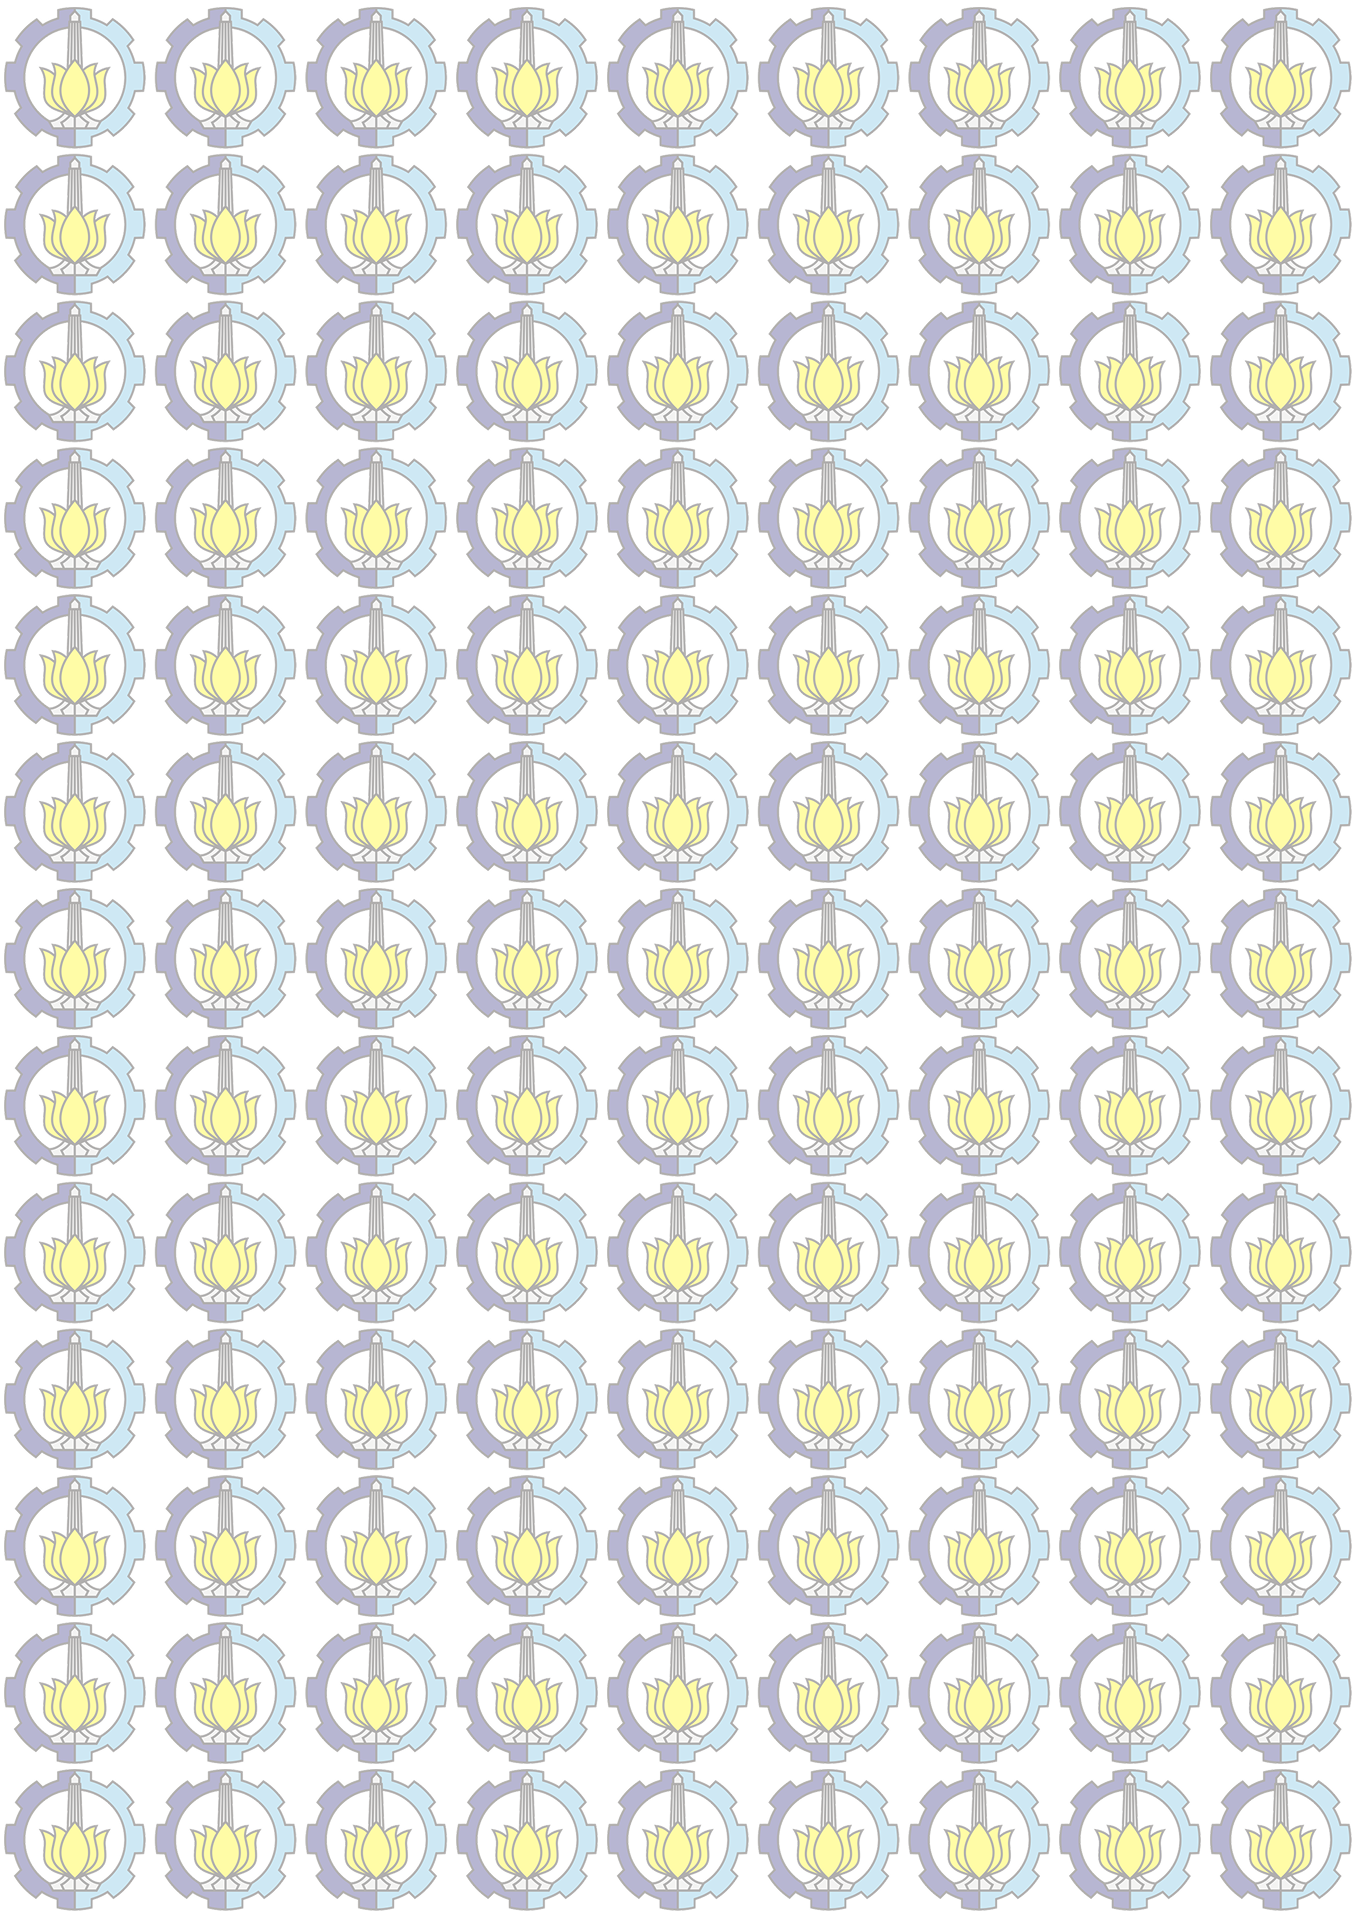
\includegraphics[width=\paperwidth]{img/watermark-a4}}
}

\renewcommand{\headrulewidth}{0pt}
\fancyhf{}
\fancypagestyle{plain}{}
\pagestyle{plain}

\newcommand{\partition}[1]{
	\vspace*{\fill}
	\vspace*{\fill}
	\vspace*{\fill}
	\begin{flushright}
		\textbf{\Huge\MakeUppercase{#1}}
	\end{flushright}
	\vspace*{\fill}
	\vspace*{\fill}
	\clearpage
}

\begin{document}
	\partition{Lembar Pengesahan}
	\partition{Pernyataan Orisinalitas}
	\partition{Abstrak}
	\partition{Abstract}
	\partition{Kata Pengantar}
	\partition{Daftar Isi}
	\partition{Daftar Gambar}
	\partition{Daftar Tabel}
	\partition{Daftar Simbol}
	\partition{Bab I  \\ [.5em] Pendahuluan}
	\partition{Bab II \\ [.5em] Tinjauan Pustaka}
	\partition{Bab III\\ [.5em] Metodologi}
	\partition{Bab IV \\ [.5em] Hasil dan Pembahasan}
	\partition{Bab V  \\ [.5em] Kesimpulan dan Saran}
	\partition{Lampiran}
	\partition{Daftar Pustaka}
	\partition{Ucapan Terima Kasih}
	\partition{Biodata Penulis}
\end{document}
